% !TEX root = ../main.tex
\subsection{Acceptance Correction} \label{ssec::acceptance_correction}
% What is acceptance
    When discussing radiation detection, it is common to describe two types of efficiency: absolute efficiency and intrinsic detection efficiency.
    The former is defined as the fraction of events emitted by the source which is actually registered by the detector, or
    \begin{equation*}
        \xi_\text{tot} = \frac{\text{events registered}}{\text{events emitted by source}}.
    \end{equation*}
    This is a function of the detector geometry and the probability of an interaction in the detector.
    Total efficiency is also known as detector acceptance.

    Then, this total efficiency can be factored into two parts: the intrinsic efficiency, $\xi_{\text{int}}$, and the geometric efficiency, $\xi_{\text{geom}}$.
    The total efficiency is then given by
    \begin{equation*}
        \xi_\text{tot} = \xi_\text{int} \cdot \xi_\text{geom}.
    \end{equation*}

    The intrinsic efficiency is that fraction of events actually hitting the detector which is registered
    \begin{equation*}
        \xi_\text{int} = \frac{\text{events registered}}{\text{events impinging on detector}}.
    \end{equation*}
    This probability depends on the interaction cross sections of the incident radiation on the detector medium.
    The intrinsic efficiency is thus a function of the type of radiation, its energy and the detector material \cite{leo1987}.

% Acceptance correction through generation + simulation.
    Acceptance correction is the process of correcting for the total efficiency of the detector.
    To obtain an estimation of this detector efficiency, we can compare the total generated events $N_\text{thrown}$ with the accepted events in a simulation of the detector $N_\text{simul}$, such that
    \begin{equation*}
        \tilde\xi_\text{tot} = \frac{N_\text{simul}}{N_\text{thrown}}.
    \end{equation*}
    This quantity is naturally dependent on the quality of the event generator and simulation programs.
    
% Chosen bins.
    Acceptance varies along the phase space of the kinematical variables.
    Thus, to make the correction accurate, the ratio must be separated into five-dimensional bins.
    These correspond to the five studied variables, $Q^2$, $\nu$, $z_h$, $p_T^2$, and $\phi_{PQ}$.
    For simplicity in analysis, all bins for a variable are of the same size, such that the results are easy to interpret.
    % The bins are designed such that there is a similar number of entries in each, with the additional requirement that the histogram curve is as linear as possible.
    \begin{itemize}
        \item
            $Q^2 = 4E_bE'\sin^2(\theta_C/2)$ is the 4-momentum transferred by the lepton probe in the lab frame, where $E_b$ is the beam energy, $E'$ is the scattered electron's energy, and $\theta_C$ is the polar angle of the scattered electron.
            % The chosen bin edges are $1.0$, $1.4$, $1.6$, $1.8$, $2.0$, $2.25$, $2.6$, $3.1$, $4.0$, and $11.0$ $\text{GeV}^2$.
            The chosen bin edges are $1$, $2$, $3$, $4$, $5$, $6$, $7$, $8$, $9$, $10$, $11.0$ $\text{GeV}^2$.
        \item
            $\nu = E_v - E'$ is the energy transferred by the lepton probe in the lab frame.
            % The chosen bin edges are $2.0$, $3.7$, $4.4$, $5.0$, $5.6$, $6.2$, $6.8$, $7.5$, $8.2$, $8.9$, and $10.1$ $\text{GeV}$.
            The chosen bin edges are $2$, $3$, $4$, $5$, $6$, $7$, $8$, $9$, and $10$ $\text{GeV}$.
        \item
            $z_h = E_h/\nu$ is the virtual photon energy fraction carried by the measured hadron, with $E_h$ being this hadron's energy.
            % The chosen bin edges are $0$, $0.11$, $0.14$, $0.17$, $0.20$, $0.23$, $0.27$, $0.32$, $0.39$, $0.50$, $0.70$, and $1$.
            The chosen bin edges are $0$, $0.1$, $0.2$, $0.3$, $0.4$, $0.5$, $0.6$, $0.7$, $0.8$, $0.9$, and $1$.
        \item
            $p_T^2$ is the hadron's transverse momentum measured with respect to the virtual photon direction.
            % The chosen bin edges are $0$, $0.06$, $0.10$, $0.14$, $0.18$, $0.24$, $0.34$, $0.60$, and $2.00$ $\text{GeV}^2$.
            The chosen bin edges are $0$, $0.2$, $0.4$, $0.6$, $0.8$, $1$, $1.2$, $1.4$, $1.6$, $1.8$, and $2$ $\text{GeV}^2$.
        \item
            $\phi_{PQ}$ is the angle between the leptonic plane -- the plane where the paths of the initial and scattered electrons lie -- and the hadronic plane, which contains the virtual photon and the measured hadron.
            % The chosen bin edges are $-180$, $-165$, $-150$, $-127.5$, $-105$, $-75$, $0$, $75$, $105$, $127.5$, $150$, $165$, and $180$ degrees.
            The chosen bin edges are $-180$, $-140$, $-100$, $-60$, $-20$, $20$, $60$, $100$, $140$, and $180$ degrees.
    \end{itemize}

    Plots for each of the variables described with vertical lines showing the bins can be seen in the plots to the left of figure \ref{fig::acc_corr}.
    The data used to obtain these plots is from RG-F run number $\mathbf{012933}$, which contains a total of $23,844,549$ reconstructed events to work with.
    % Considering the defined bin edges, we have a total of $9 \cdot 10 \cdot 8 \cdot 11 \cdot 12 = 95,040$ bins, leaving us a measly $250.8$ events per bin. % TODO. WHAT TO DO ABOUT THESE? JUST LESS BINS?

    To compute the acceptance, 10 million events were generated in deep inelastic kinematics using LEPTO, a Monte Carlo generator for deep inelastic lepton-nucleon scattering \cite{ingelman1997}.
    Then, the events were simulated in the RG-F experiments conditions in CLAS12 by using \texttt{gemc}, with a torus field polarity of $-1$ and solenoid field polarity of $-0.745033$.
    \texttt{gemc} is the standard tool used for simulating CLAS12 events \cite{ungaro2020gemc}.
    Finally, they were reconstructed using \texttt{coatjava}, the standard tool for CLAS12 event offline reconstruction \cite{ziegler2020}.
    A description of the last can be read in section \ref{sssec::offlinereconstruction}.

% Acceptance correction results.
    The plots to the right of figure \ref{fig::acc_corr} show the number of generated events in red and the number of simulated events that were successfully reconstructed out of that set in blue.
    Each one is presented in integrated kinematical region for the other variables.
    As described before, the acceptance correction factor comes from the quotient of the number of simulated events, $N_\text{simul}$ versus the number of thrown events, $N_\text{thrown}$.
    
% Plots.
    \begin{figure}[hbtp]
        % Q2.
        \begin{subfigure}{.5\textwidth}
            \centering
            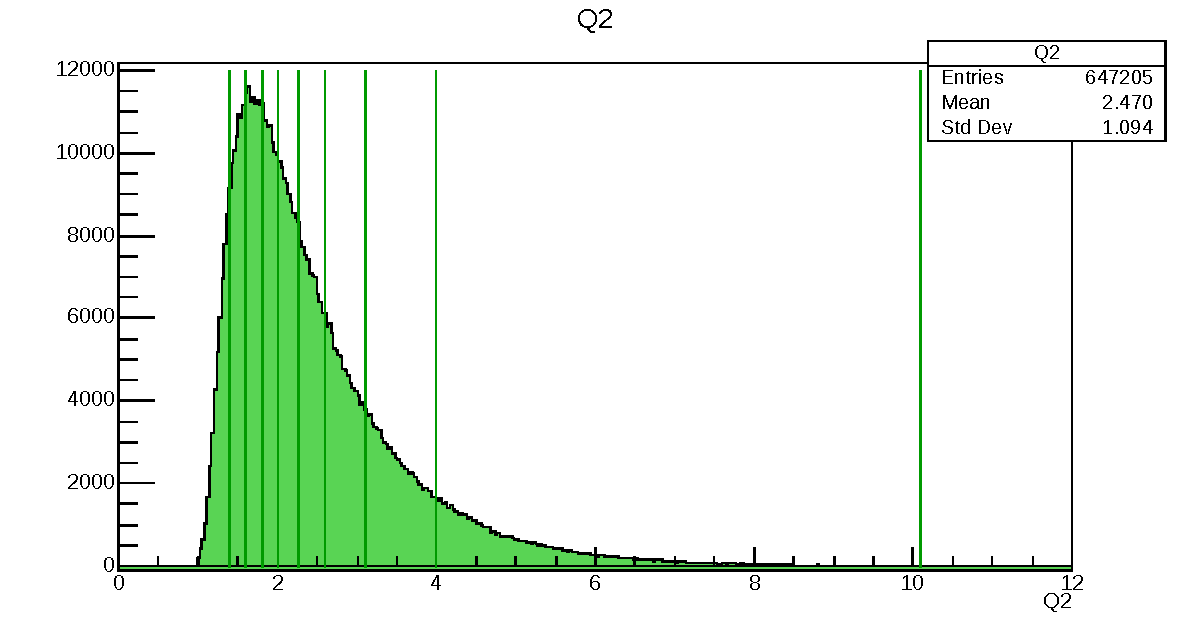
\includegraphics[width=\linewidth]{13dataanalysis/img/40_accbins_q2.pdf}
            % \caption{$Q^2$ bins.}
            \label{fig::acc_corr_bins_q2}
        \end{subfigure}
        \begin{subfigure}{.5\textwidth}
            \centering
            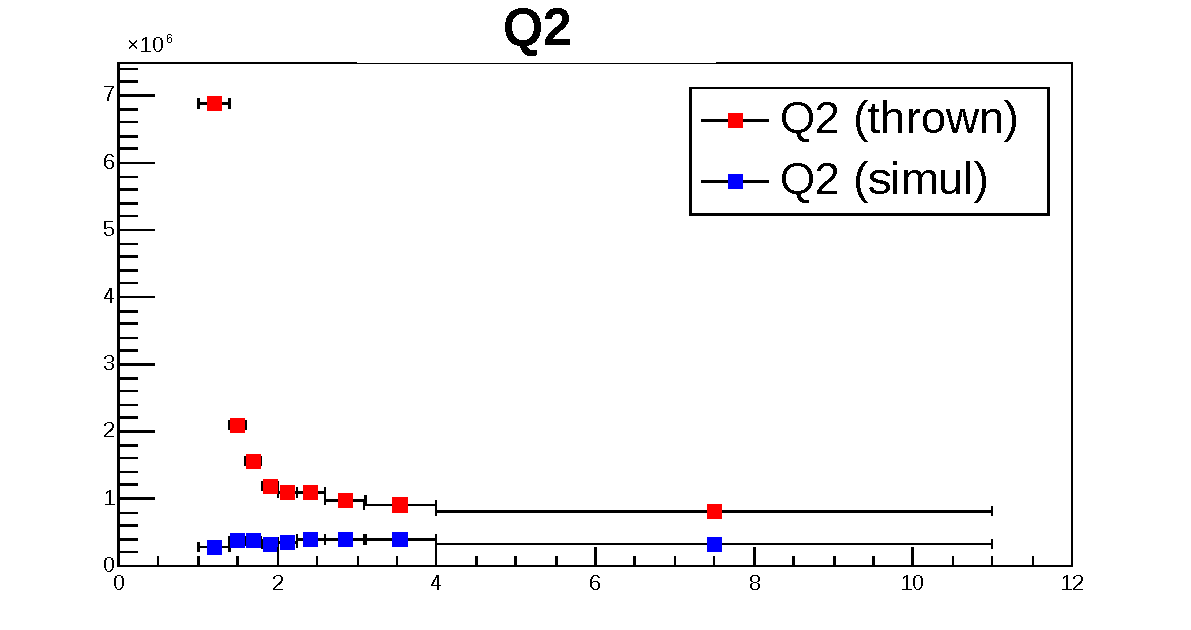
\includegraphics[width=\linewidth]{13dataanalysis/img/40_acccorr_q2.pdf}
            % \caption{$Q^2$ acceptance correction results.}
            \label{fig::acc_corr_q2}
        \end{subfigure}

        % nu.        
        \begin{subfigure}{.5\textwidth}
            \centering
            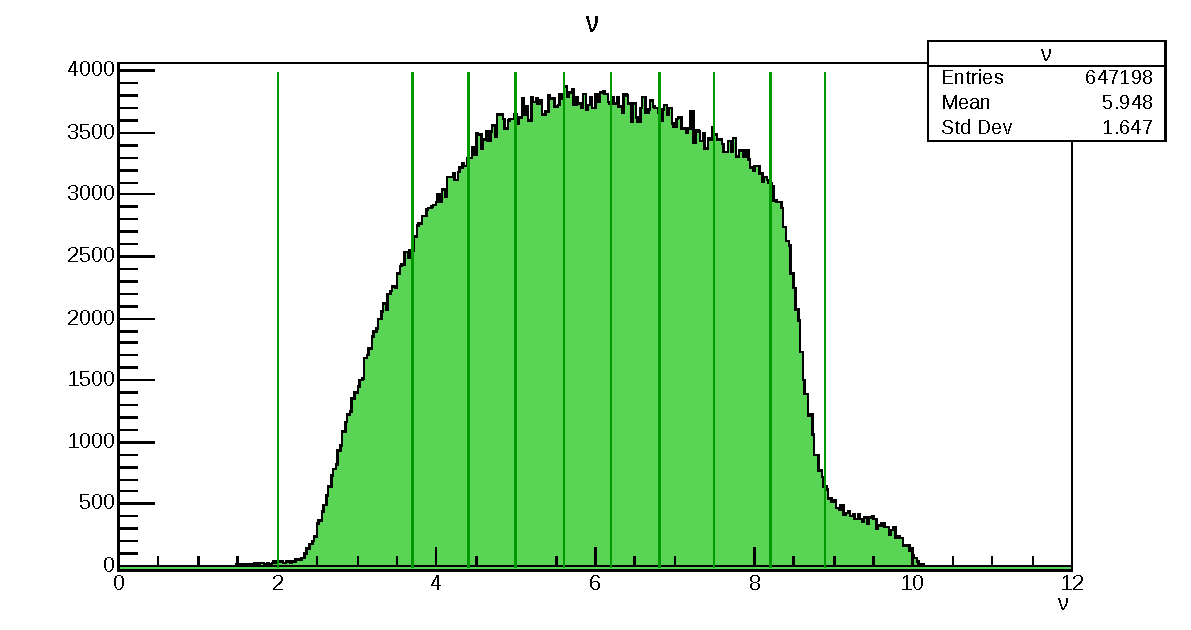
\includegraphics[width=\linewidth]{13dataanalysis/img/40_accbins_nu.pdf}
            % \caption{$\nu$ bins.}
            \label{fig::acc_corr_bins_nu}
        \end{subfigure}
        \begin{subfigure}{.5\textwidth}
            \centering
            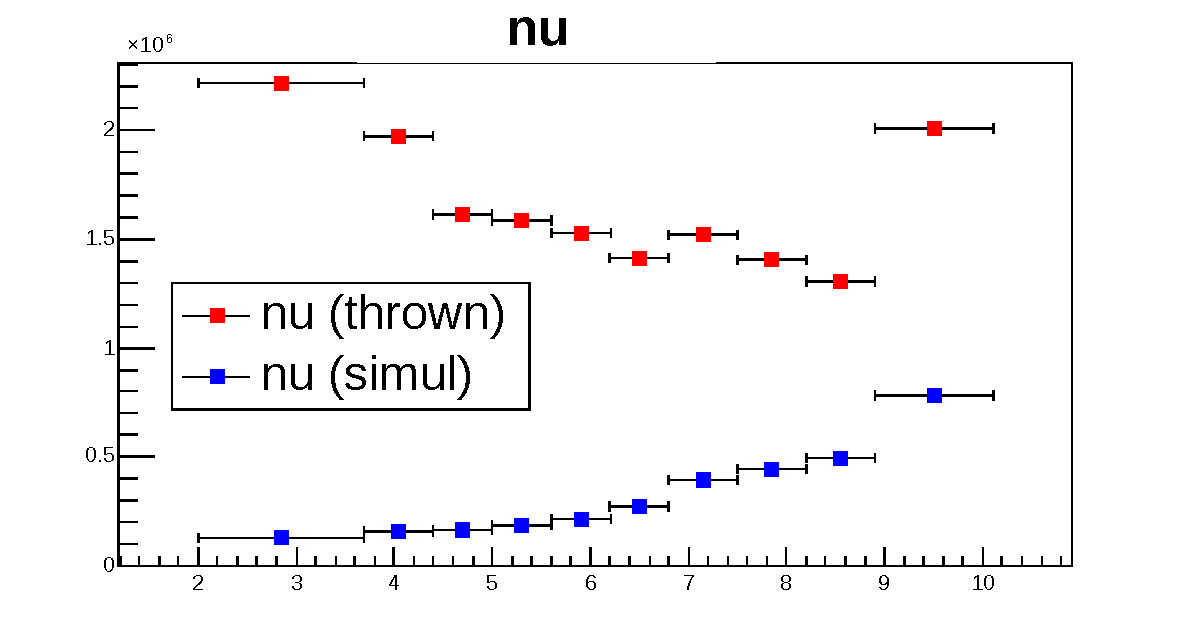
\includegraphics[width=\linewidth]{13dataanalysis/img/40_acccorr_nu.pdf}
            % \caption{$\nu$ acceptance correction results.}
            \label{fig::acc_corr_nu}
        \end{subfigure}

        % zh.
        \begin{subfigure}{.5\textwidth}
            \centering
            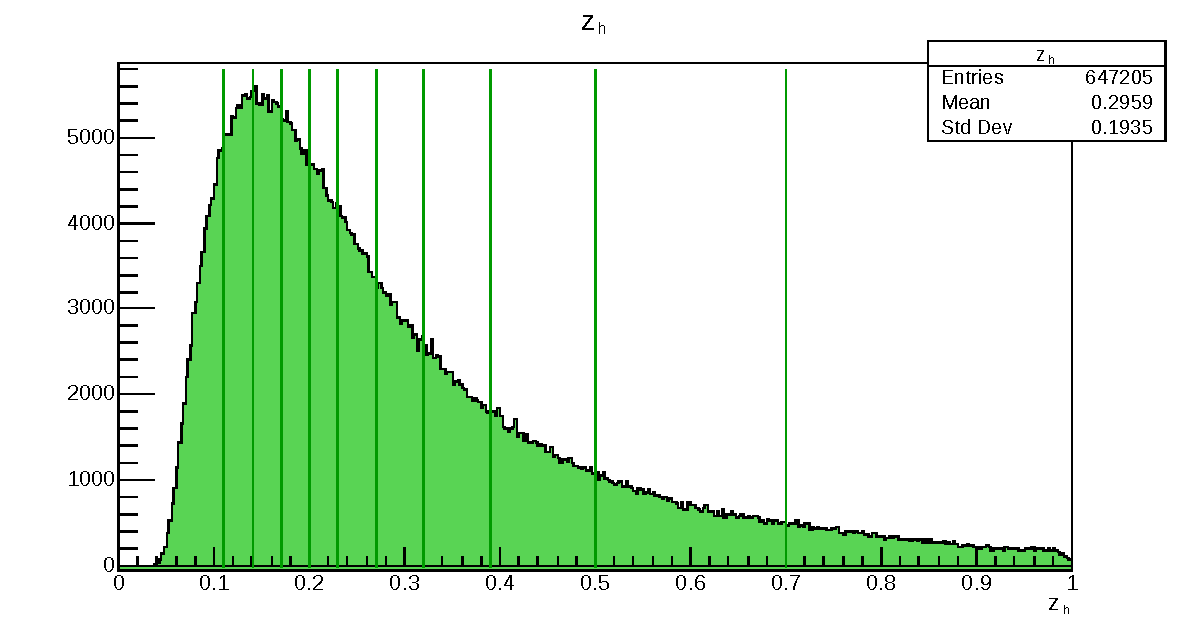
\includegraphics[width=\linewidth]{13dataanalysis/img/40_accbins_zh.pdf}
            % \caption{$z_h$ bins.}
            \label{fig::acc_corr_bins_zh}
        \end{subfigure}
        \begin{subfigure}{.5\textwidth}
            \centering
            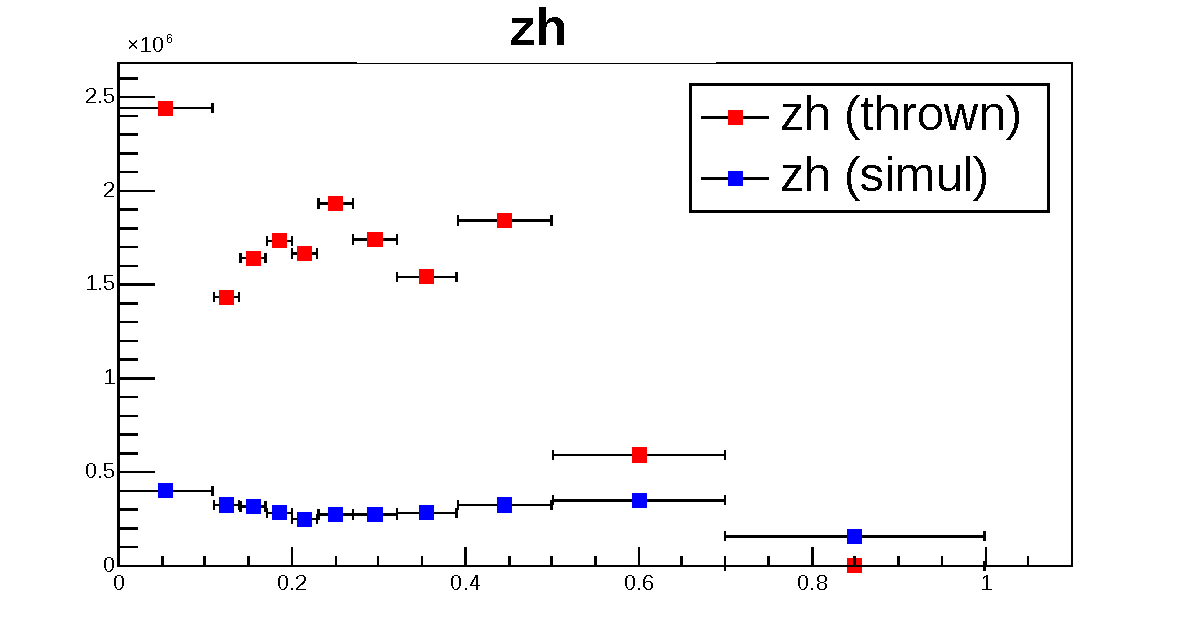
\includegraphics[width=\linewidth]{13dataanalysis/img/40_acccorr_zh.pdf}
            % \caption{$z_h$ acceptance correction results.}
            \label{fig::acc_corr_zh}
        \end{subfigure}

        % PT2.
        \begin{subfigure}{.5\textwidth}
            \centering
            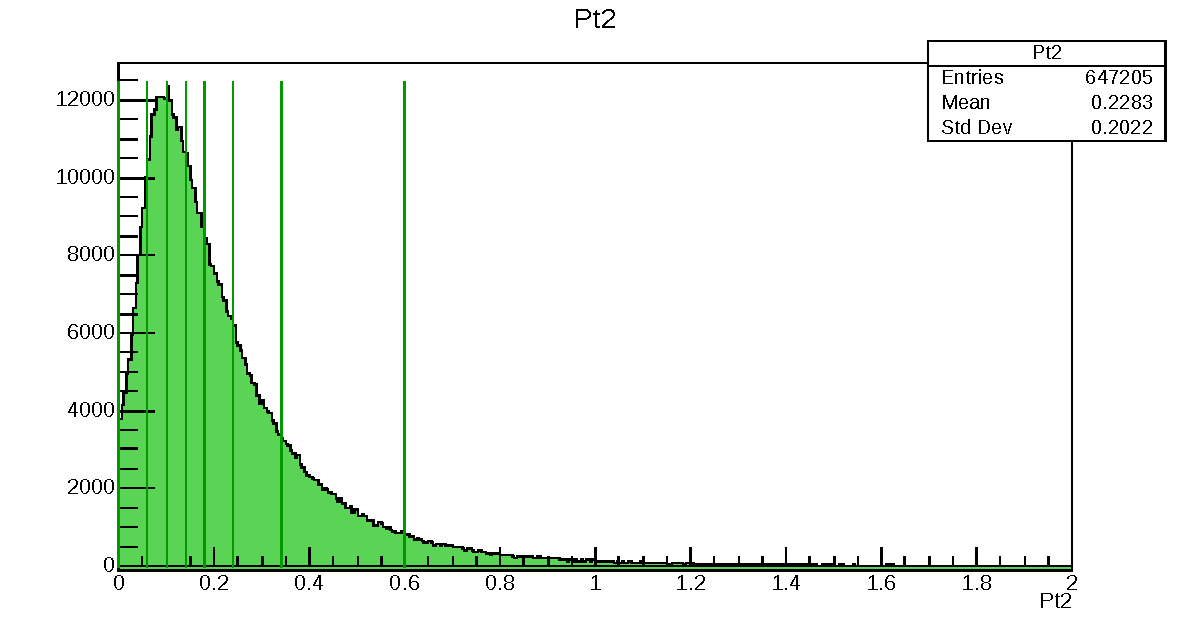
\includegraphics[width=\linewidth]{13dataanalysis/img/40_accbins_pt2.pdf}
            % \caption{$P_T^2$ bins.}
            \label{fig::acc_corr_bins_pt2}
        \end{subfigure}
        \begin{subfigure}{.5\textwidth}
            \centering
            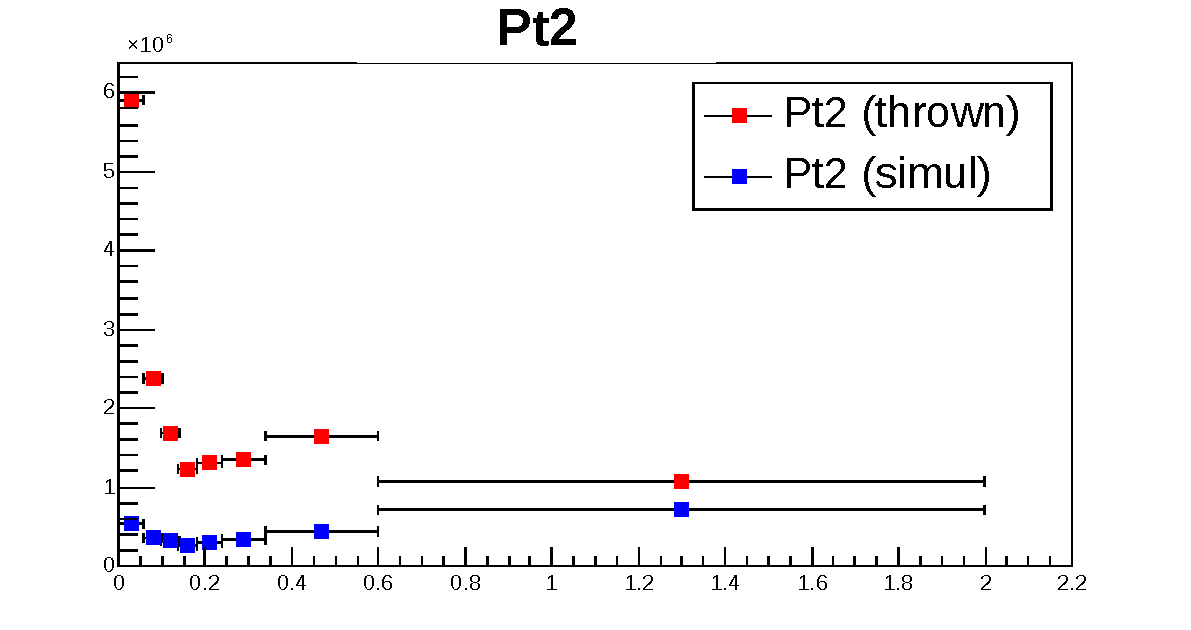
\includegraphics[width=\linewidth]{13dataanalysis/img/40_acccorr_pt2.pdf}
            % \caption{$P_T^2$ acceptance correction results.}
            \label{fig::acc_corr_pt2}
        \end{subfigure}

        % phi_PQ.
        \begin{subfigure}{.5\textwidth}
            \centering
            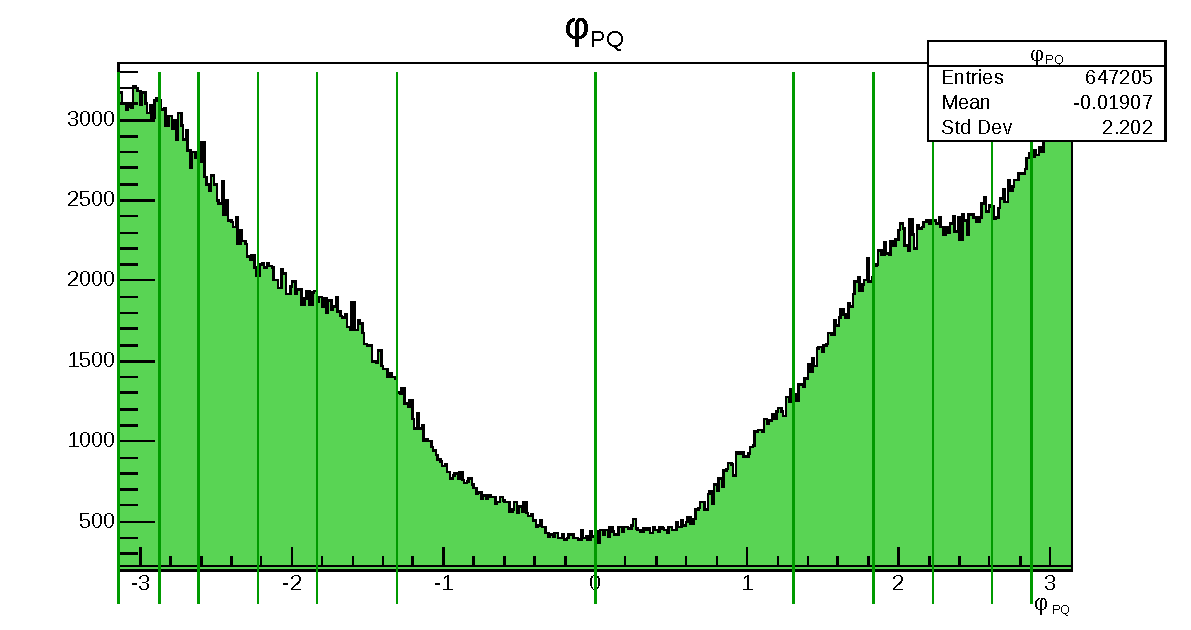
\includegraphics[width=\linewidth]{13dataanalysis/img/40_accbins_phipq.pdf}
            % \caption{$\phi_{PQ}$ bins.}
            \label{fig::acc_corr_bins_phipq}
        \end{subfigure}
        \begin{subfigure}{.5\textwidth}
            \centering
            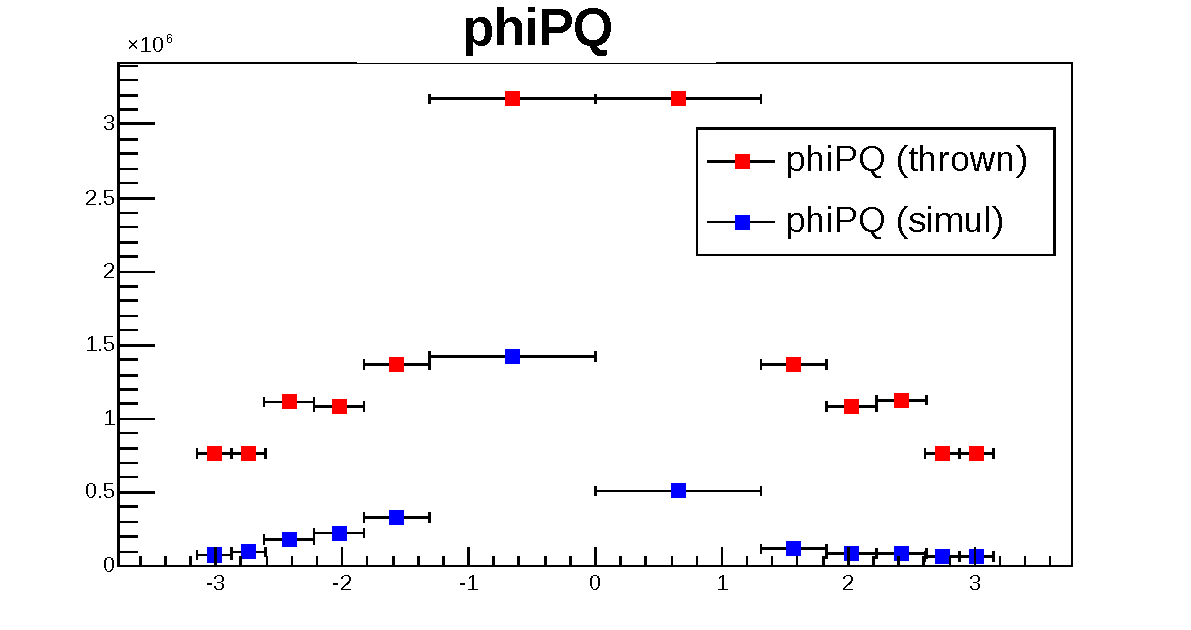
\includegraphics[width=\linewidth]{13dataanalysis/img/40_acccorr_phipq.pdf}
            % \caption{$\phi_{PQ}$ acceptance correction results.}
            \label{fig::acc_corr_phipq}
        \end{subfigure}

        \caption[Acceptance correction results.]{Acceptance correction results for the kinematical variables $Q^2$, $\nu$, $z_h$, $p_T^2$, and $\phi_{PQ}$. On the left plots, the acceptance correction bin edges are shown. On the right, the number of thrown (in red) and simulated (in blue) entries for each of the variables is shown. All other variables are integrated for each plot.}
        \label{fig::acc_corr}
    \end{figure}
